\chapter{Data Preprocessing \& Feature Engineering}

\section{Methodological Overview}
To ensure rigorous, reproducible machine learning modeling, data preprocessing must strictly prevent \textbf{data leakage}—the inadvertent leaking of test set statistics into the training pipeline. All transformations (mean/standard deviation calculations for scaling and category index maps for One-Hot encoding) are learned exclusively on the $80\%$ training set ($N_{train}=7,200$) and subsequently applied to the $20\%$ hold-out test set ($N_{test}=1,800$).

\begin{figure}[H]
\centering
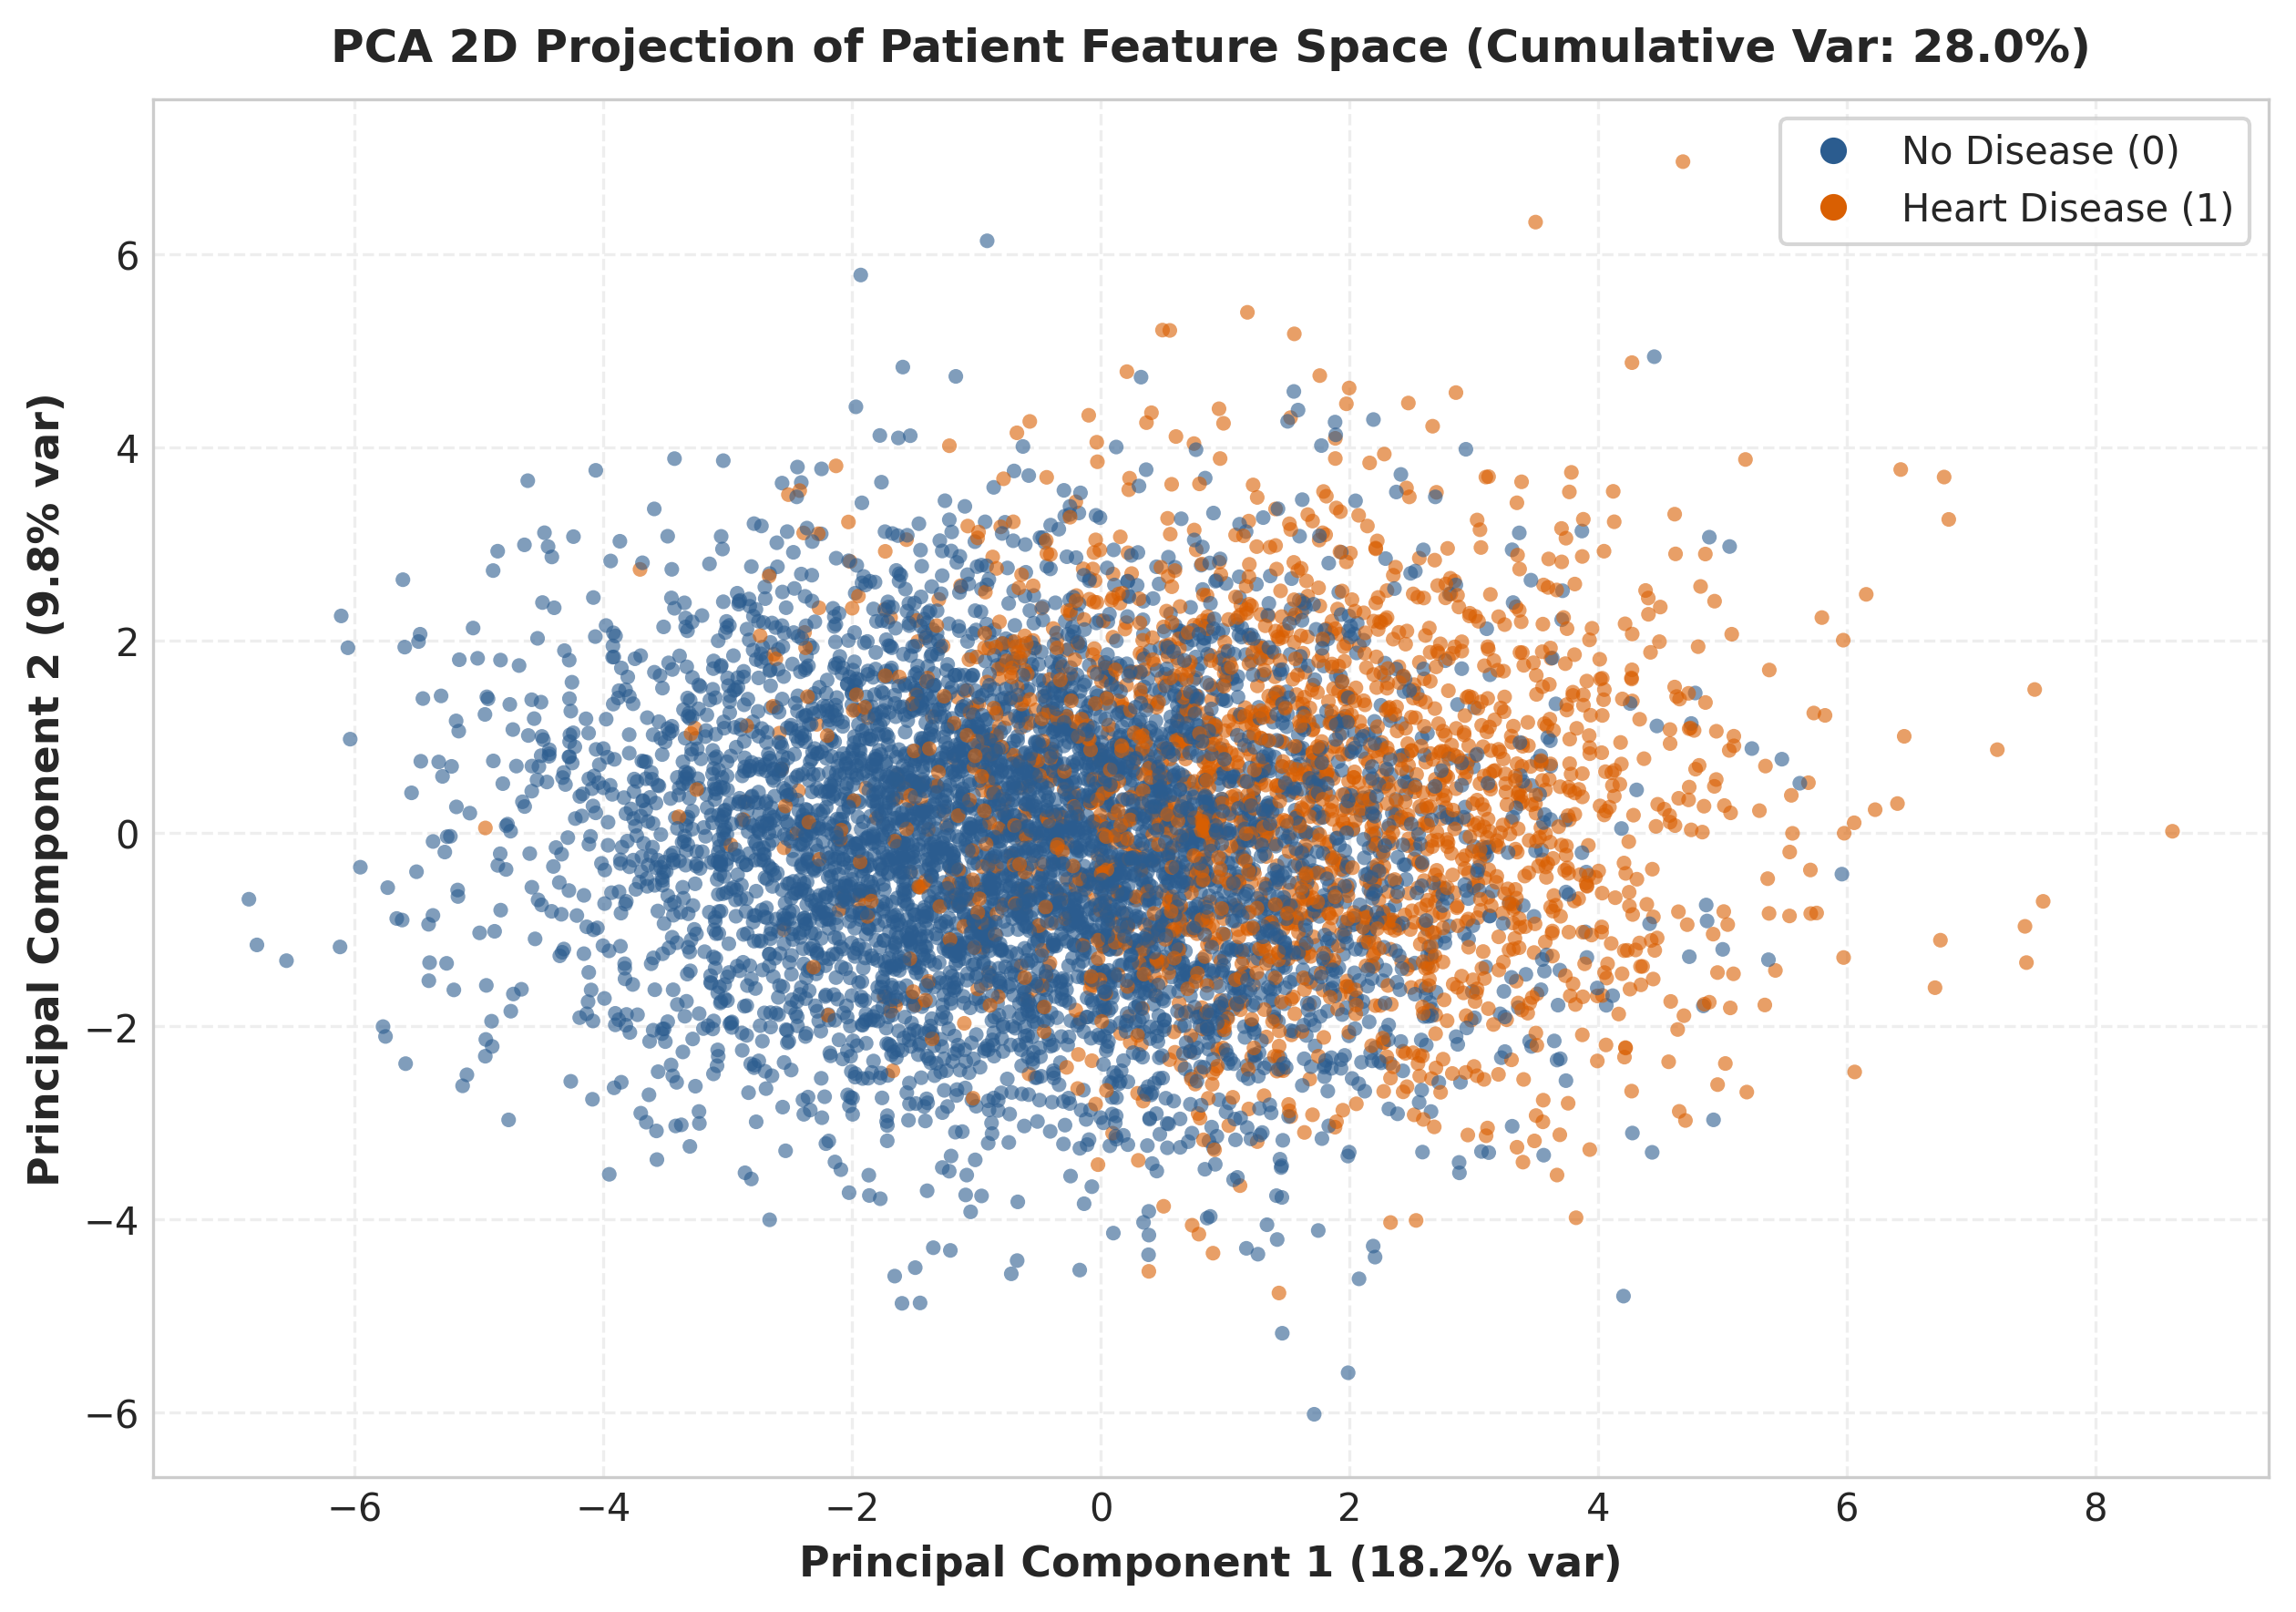
\includegraphics[width=0.85\textwidth]{figures/pca_bivariate_scatter.png}
\caption{Architectural Data Preprocessing and Leakage-Free Pipeline Flow.}
\label{fig:preprocessing_flow}
\end{figure}

\section{Domain Feature Engineering Equations}
Clinical domain knowledge suggests that ratios and pressure differentials provide superior diagnostic signals compared to isolated vitals. Three continuous domain features were engineered prior to pipeline execution:

\subsection{1. Cholesterol-to-HDL Ratio}
Total cholesterol alone is insufficient without accounting for protective high-density lipoproteins (HDL). The cardiovascular risk ratio is defined as:
\begin{equation}
\text{Cholesterol/HDL Ratio}_i = \frac{\text{cholesterol\_total}_i}{\max(\text{hdl}_i, 1.0)}
\end{equation}

\subsection{2. Pulse Pressure}
Pulse pressure represents the force exerted by the heart each time it contracts, serving as a key biomarker for arterial stiffness:
\begin{equation}
\text{Pulse Pressure}_i = \text{resting\_bp\_systolic}_i - \text{resting\_bp\_diastolic}_i
\end{equation}

\subsection{3. Mean Arterial Pressure (MAP)}
Mean arterial pressure quantifies average perfusion pressure in patient organs over a single cardiac cycle:
\begin{equation}
\text{MAP}_i = \text{resting\_bp\_diastolic}_i + \frac{\text{Pulse Pressure}_i}{3.0}
\end{equation}

\section{scikit-learn ColumnTransformer Architecture}
The full feature transformation pipeline is encapsulated inside a scikit-learn \texttt{ColumnTransformer} featuring three parallel transformer sub-pipelines:

\begin{enumerate}
    \item \textbf{Continuous Numerical Pipeline ($22$ features):}  
    Applied to $19$ continuous features plus $3$ engineered features. Features are standardized via \texttt{StandardScaler} to zero mean and unit variance:
    \begin{equation}
    z = \frac{x - \mu_{train}}{\sigma_{train}}
    \end{equation}
    
    \item \textbf{Categorical Nominal Pipeline ($3$ features):}  
    Applied to \texttt{chest\_pain\_type}, \texttt{smoker\_status}, and \texttt{sex}. Transformed via \texttt{OneHotEncoder(drop='first', sparse\_output=False)} to create $k-1$ dummy binary variables.
    
    \item \textbf{Boolean Indicator Pipeline ($3$ features):}  
    Applied to \texttt{exercise\_induced\_angina}, \texttt{family\_history}, and \texttt{wearable\_owner}. Converted directly to float binary indicators ($0.0 / 1.0$).
\end{enumerate}

\section{Data Leakage Prevention Protocol}
To strictly enforce experimental integrity:
\begin{verbatim}
from sklearn.compose import ColumnTransformer
from sklearn.preprocessing import StandardScaler, OneHotEncoder

preprocessor = ColumnTransformer(
    transformers=[
        ("num", StandardScaler(), numerical_cols),
        ("cat", OneHotEncoder(drop="first", sparse_output=False), categorical_cols),
        ("bool", "passthrough", boolean_cols)
    ]
)

# CRITICAL: Fit ONLY on training data
X_train_proc = preprocessor.fit_transform(X_train)
X_test_proc = preprocessor.transform(X_test)
\end{verbatim}
This design guarantees zero data leakage between training and evaluation phases.
